\sloppy
%
% JaCa-Android guide
%
\documentclass[11pt]{report}
\usepackage{url}
 \newif\ifpdf
 \ifx\pdfoutput\undefined
 \pdffalse % we are not running PDFLaTeX
 \else
 \pdfoutput=1 % we are running PDFLaTeX
 \pdftrue
 \fi
%%%%%%%%%%%%%%%
 \ifpdf
 \usepackage[pdftex]{graphicx}
 \else
 \usepackage{graphicx}
 \fi
%%%%%%%%%%%%%%%
 \ifpdf
 \DeclareGraphicsExtensions{.pdf, .jpg, .tif}
 \else
 \DeclareGraphicsExtensions{.eps, .jpg}
 \fi
%%%%%%%%%%%%%%%

\graphicspath{{./images/}}

\newcommand\xc[1]{\chaptername~\ref{chap:#1}}
\newcommand\labelchap[1]{\label{chap:#1}}
\newcommand\xa[1]{\appendixname~\ref{app:#1}}
\newcommand\labelsec[1]{\label{sec:#1}}
\newcommand\xs[1]{\sectionname~\ref{sec:#1}}
\newcommand\xsp[1]{\sectionname~\ref{sec:#1} \onpagename~\pageref{sec:#1}}
\newcommand\labelssec[1]{\label{ssec:#1}}
\newcommand\xss[1]{\subsectionname~\ref{ssec:#1}}
\newcommand\xssp[1]{\subsectionname~\ref{ssec:#1} \onpagename~\pageref{ssec:#1}}
\newcommand\labelsssec[1]{\label{sssec:#1}}
\newcommand\xsss[1]{\subsectionname~\ref{sssec:#1}}
\newcommand\xsssp[1]{\subsectionname~\ref{sssec:#1} \onpagename~\pageref{sssec:#1}}
\newcommand\labelfig[1]{\label{fig:#1}}
\newcommand\xf[1]{\figurename~\ref{fig:#1}}
\newcommand\xff[2]{\figurenames~\ref{fig:#1}~and~\ref{fig:#2}}
\newcommand\xfp[1]{\figurename~\ref{fig:#1} \onpagename~\pageref{fig:#1}}
\newcommand\labeltab[1]{\label{tb:#1}}
\newcommand\xt[1]{\tablename~\ref{tb:#1}}
\newcommand\xtt[2]{\tablenames~\ref{tb:#1}~and~\ref{ab:#2}}
\newcommand\xtp[1]{\tablename~\ref{tb:#1} \onpagename~\pageref{tb:#1}}
\newcommand\labelenum[1]{\label{enum:#1}}
\newcommand\xen[1]{(\ref{enum:#1})}
\newcommand\xenp[1]{(\ref{enum:#1}) \onpagename~\pageref{enum:#1}}
%\newcommand{\chaptername}{Chapter}
%\newcommand{\figurename}{Figure}
%\newcommand{\tablename}{Table}
\newcommand{\sectionname}{Section}

%******************************************************************************%
\newcommand\note[1]{NOTE:\emph{#1}}
\newcommand\tbc[1]{TO BE COMPLETED: \emph{#1}}
\newcommand\outd[1]{OUTDATED: \emph{#1}}
\newcommand\tbd[1]{TO BE COMPLETED: \emph{#1}}
\newcommand\code[1]{{\mbox{\texttt{{#1}}}}}
\newcommand\keyword[1]{{\mbox{\textsf{{#1}}}}}
\newcommand\sym[1]{{\small{\mbox{\textit{{#1}}}}}}
\newcommand\ttit[1]{\texttt{\textit{#1}}}

\newcommand\version[1]{\mbox{Document revision: #1}}
\newcommand\approvedby[1]{\mbox{Approved by: #1}}
\newcommand\receivedby[1]{\mbox{Received by: #1}}
\newcommand\creationdate[1]{\mbox{Creation date: #1}}
\newcommand\repauthor[1]{\mbox{Main author: #1}}
\newcommand\lastchangesdate[1]{\mbox{Last Changes date: #1}}
\newcommand\noa[2]{\noindent\emph{Note of the author (#1): }#2\\\\}
\newcommand\logo{
    \begin{figure}[tp]
        \begin{center}
            \inputgraphics[width=4cm]{../shared/logo}
        \end{center}
\end{figure}}

%******************************************************************************%
\newcommand{\jacandroidversion}{2.0}
\newcommand{\jaca}{\mbox{\sf{JaCa}}}
\newcommand{\jason}{\mbox{\sf{\emph{{Jason}}}}}
\newcommand{\AandA}{\mbox{\sf{{A\&A~}}}}
\newcommand{\cartago}{\mbox{\sf{CArtAgO}}}
\newcommand{\jacandroid}{\textsf{JaCa-Android}}

%******************************************************************************%

\title{{\huge{\bf{{\jacandroid} By Example}}\\~\\\mbox{version: \jacandroidversion{}}\\\mbox{~}\\}
{\small{
   \repauthor{asanti}  \\  
    \creationdate{20110331}\\
    \lastchangesdate{20110411}\\
    % \receivedby{aricci}\\
    % \approvedby{aricci}\\
    }}
}

\author{DEIS, Universit\`{a} di Bologna, Italy}

\date{}

\begin{document}

\maketitle
\sloppy

\tableofcontents

\chapter{Introduction}
In the following we describe some main features of \jacandroid{} making a sequence of simple tests, example and performance tests focussing on the different functionalities provided by the middleware.
%
This document is meant to be read by people already familiar with the \jaca{} programming model---the programming model upon which \jacandroid{} is based. If you are an inexperienced reader please consider to acquire a good background knowledge on both \cartago{} and \jason{} and in the \jaca{} programming model (raw speaking the synergistic integration of these two agent-based technologies). The quickest way for getting started with the \jaca{} programming model is the \cartago{} by example tutorial that can be found on the \cartago{} website\footnote{\url{http://cartago.sourceforge.net/?page_id=47}}. For more exhaustive informations the following references can be considered:

\begin{itemize}
	\item The \jason{} book\cite{bhw07}, the reference \jason{} paper \cite{jason06} and the \jason{} website\footnote{\url{http://jason.sourceforge.net/}}.
	\item Some papers about \cartago{}\cite{cartago:jaamas08,cartago09map,cartago-e4masIII} and the \cartago{} website\footnote{\url{http://www.cartago.sourceforge.net}}.
\end{itemize}

All the examples that we describe in this document are packed together in a simple Android application (the \jacandroid{} sample suite) that can be used for testing the examples in your device. The \code{.apk} containing the examples (named \textsf{JaCa-Android-Samples.apk}) can be found inside the \code{Apk} folder placed in the root of the standard \jacandroid{} distribution. The folder \code{JaCa-Android-Samples} contains instead the test suite sources. This folder is also a \jacandroid{} Eclipse project that can be directly imported into your workspace.
%
For running the samples in your device is required that you first install and configure the \jacandroid{} middleware, instructions for doing this can be found in the getting started guide\footnote{\url{http://jaca-android.sourceforge.net/?page_id=257}}.

\chapter{Tests}

In this chapter we describe a set of examples useful to highlight the basic use of the main functionalities provided by the \jacandroid{} middleware. You can find the source code of this samples inside the \code{JaCa-Andorid-Samples/src/tests} folder. For running the samples just install the \textsf{JaCa-Android-Samples.apk}, launch the application, choose \textsf{JaCa-Android Tests} and the select the sample you want to launch.
%
\begin{figure}[h!]
\begin{center}
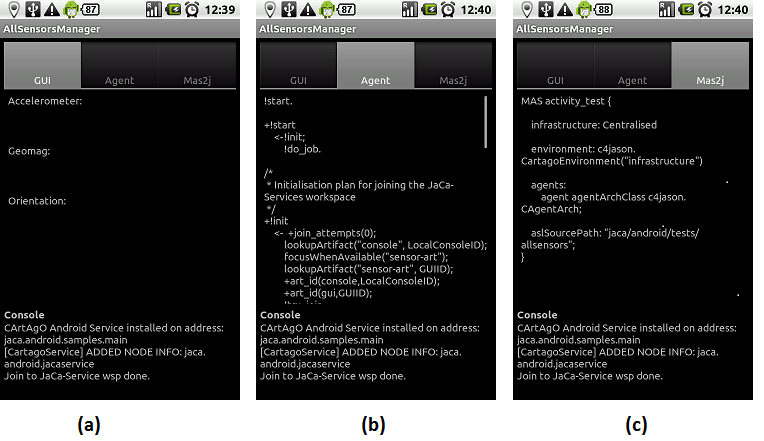
\includegraphics[width=.9\linewidth]{images/example_gui.png}
\end{center}
\caption{The GUI structure of the examples considered in this chapter.}
\labelfig{gui-samples}
\end{figure}

All the samples contained in the \code{tests} folder have been realised using the same structure for the GUI, showed in \xf{gui-samples}, where you can see: \textit{(i)} a tab containing the specific GUI (\xf{gui-samples} (a)) of the application (if present), \textit{(ii)} a tab containing the source code of the agent used in that example (\xf{gui-samples} (b)), \textit{(iii)} a tab containing the \code{\textsf{mas2j}} configuration file (\xf{gui-samples} (c)), and on the bottom \textit{(iv)} a output console in which is possible to see output and error messages. In most of the samples the agents used have an initialisation plan (the \code{init} plan), not reported in this document for simplicity, exploited for joining the \textsf{MiddlewareServices} shared workspace. For fully understand how to join remote workspaces of other \jacandroid{} applications please refer to the example reported in \xs{remotewsp-android}.



\section{Example 01 - Working with GUI}

Before going in the details of this first example we provide a basic description of the \textsf{GUIArtifact}, the basic artifact used for managing an Android GUI in \jacandroid{}.


\subsection{The \textsf{GUIArtifact}}
The \textsf{GUIArtifact} is the basic artifact used for managing an Android GUI in \jacandroid{}.
%
This artifact wraps a real Android GUI using a \textsf{\textsf{IJaCaActivity}} -- which is an interface part of our middleware representing a \jacandroid{} extension of an Android GUI base class  -- for providing developers a connection between the concrete GUI and the artifact that manages it.
%
Thanks to the \textsf{\textsf{IJaCaActivity}} it is hence possible to manipulate the Android GUI directly from the artifact---e.g. see what we have done in the getting started example\footnote{\url{http://jaca-android.sourceforge.net/?page_id=257}} where inside the \code{addSMSToList} operation of the \textsf{ViewerArtifact} we added a new SMS to a list displayed in the smart-phone screen.

%
This artifact has only one observable property (\code{state}) representing the current state of the GUI, and provides a set of built-in mechanisms (i.e. protected methods \code{linkOnStartEventToOp}, \code{linkOnTouchEventToOp}, etc.) for linking each kind of GUI-related Android event to the artifact operation responsible of the managing of such event.
%
In the artifact initialisation -- once the linking between events and operations has been made -- is executed an internal operation (\code{execInternalOp("fetchGUIEvents");}) that manages the notification of Android GUI events. This operation is meant to \textit{cyclically}: \textit{(i)} wait for new events and \textit{(ii)} call the appropriate artifact operation (using the primitive \code{execInternalOp}).

%
The \textsf{GUIArtifact} cannot be directly used for realising a GUI in \jacandroid{}. For concretely realise an artifact-based GUI we need to specialise the \textsf{GUIArtifact} (like in the case of the \textsf{ViewerArtifact} in the getting started): \textit{(i)} explicitly defining the links between events and operations we are interested in, \textit{(ii)} wrapping the specific \textsf{IJaCaActivity} -- i.e. the GUI -- we want to manage.
%

\subsection{The sample}
In this first example we will show how to work with GUI in \jacandroid{} through the classic hello world example. You can find the source code of this example in the folder \code{/jaca/android/tests/gui} placed inside the main \code{tests} folder. The GUI used in this example is composed of three different tabs (wrapped in three different artifacts), each one of them contains a \code{print} button that once clicked will produce in standard output the following message: \code{Hello World from X}, where \code{X} is the identifier of the Artifact used to discriminate the tab the user was in when he pressed the \code{print} button.


\begin{table}[!h]
\begin{tabular} {p{10cm}}
\begin{minipage}{10cm}

{\scriptsize \begin{verbatim}
public class HelloWorldGUIArtifact extends GUIArtifact{

  protected void init(JaCaActivity activity, Bundle savedInstanceState) {
    super.init(activity, savedInstanceState);
    linkOnStartEventToOp("onStart");
    linkOnStopEventToOp("onStop");
    Button btnInc = (Button) activity.findViewById(R.id.btnPrint);
    linkOnClickEventToOp(btnInc, "onClick");
  }
	
  @OPERATION void print() {
    System.out.println("Hello World from: "+getId().getName());
  }
	
  @INTERNAL_OPERATION void onClick(View view) {
    signal(getId().getName());
  }
	
  @INTERNAL_OPERATION void onStart() {
    signal("onStart");
  }
    
  @INTERNAL_OPERATION void onStop() {
    signal("onStop");
  }
  ...
}
\end{verbatim}}
\end{minipage}
\end{tabular}
\caption{Source code snippet of the \textsf{HelloWorldGUIArtifact}.}
    \labeltab{HelloWorldGUIArtifact}
\end{table}

In this example we will use three instance of the \textsf{HelloWorldGUIArtifact}, each one representing one tab of our sample, extending the base \textsf{GUIArtifact} class. 

In \xt{HelloWorldGUIArtifact} is reported a source code snippet of the \textsf{HelloWorldGUIArtifact}.
%
\textsf{HelloWorldGUIArtifact} highlights:
\begin{itemize}
%
\item In the artifact initialisation the protected methods \code{linkOnXXXEventToOp} are used for linking the execution of
artifact's internal operations: \textit{(i)} to the occurrence of Android events, and \textit{(ii)} to the corresponding actions that the user can do on the GUI (\code{linkOnClickEventToOp(btnInc,"onClick")} for linking the execution of the \code{onClick} internal operation to clicks on the print buttons).
%
\item In the \code{onClick} internal operation the \textsf{HelloWorldGUIArtifact} emits a signal (perceivable by agents that are observing the artifact) containing the name of the artifact identifying the tab. The name of the artifact is retrieved by the \code{getId()} method inherited from the \code{Artifact} base class.
%
\item The other internal operations generate signals indicating the occurrence of particular Android events (\code{onStart}, \code{onStop}, etc.).
%	
\end{itemize}


\begin{table}[!ht]
\begin{tabular} {p{10cm}}
\begin{minipage}{10cm}
{\scriptsize \begin{verbatim}
!init.

+!init 
  <-  lookupArtifact("workspace", Id);
		  focus(Id);
		  println("init done").

+state(State) [artifact_name(_,X)]
  <-  println("state  ", X, " :", State).

+onStart [artifact_name(_,X)]
  <-  println("onStart ", X).

+onStop [artifact_name(_,X)]
  <-  println("onStop ", X).

  ...

+artifact("first_activity", _, Id)
  <-  println("first activity created"); 
      focus(Id).

+artifact("second_activity", _, Id)
  <-  println("second activity created"); 
      focus(Id).
  ...	
  
+first_activity
  <-  print [artifact_name("first_activity")].
	
+second_activity
  <-  print [artifact_name("second_activity")].
	
+third_activity
  <-  print [artifact_name("third_activity")].
\end{verbatim}}
\end{minipage}
\end{tabular}
\caption{Source code snippet of the \jason{} agent used in this test.}
    \labeltab{test0agent}
\end{table}

In \xt{test0agent} is reported the source code of the agent used in this first example.
%
Agent highlights:
\begin{itemize}
%	
\item The agent has a \code{init} plan where it lookups and focuses the workspace artifact. In this way, each time a new artifact is created in the workspace the agent is able to receive the \code{+artifact(Name, Template, Id)} event.
%	
\item The \code{+artifact(Name, Template, Id)} event is handled by a set of reactive plans that the agent uses for starting focusing each	\textsf{HelloWorldGUIArtifact} as soon as it is created.
%	
\item When a click on the GUI buttons is performed by the user the corresponding \textsf{HelloWorldGUIArtifact} generates a signal that is handled by a proper reactive plan of the agent (\code{+first\_activity} in case of signal coming from the first \textsf{HelloWorldGUIArtifact}, \code{+second\_activity} in case of signal coming from the second \textsf{HelloWorldGUIArtifact}, etc.) where the \code{print} operation of the \textsf{HelloWorldGUIArtifact} is used for printing in the \code{console} the Hello World message.
\end{itemize}


\begin{figure}[!ht]
\begin{center}
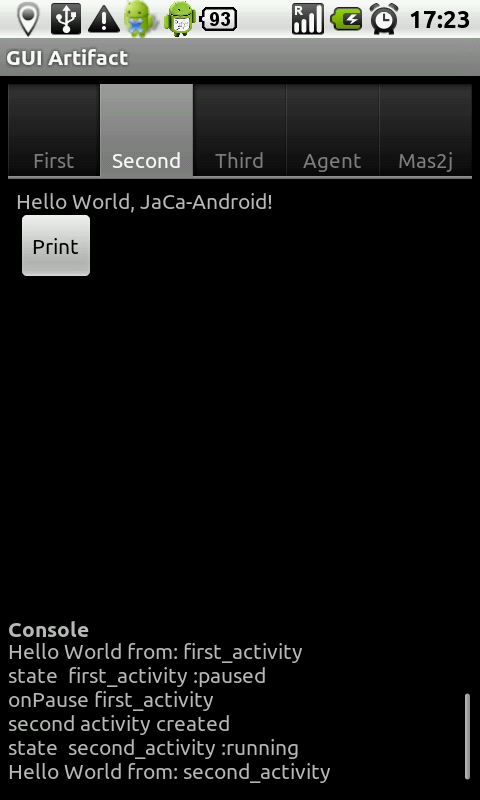
\includegraphics[width=6cm]{images/test_gui_gui.png}
\end{center}
\caption{A screenshot of the described sample.}
\end{figure}


We know that at first glance the dynamic just described could seems a bit tricky. Actually it is, but we realised this example in order to show you: \textit{(i)} the linking of artifacts' operations to both GUI and Android events and \textit{(ii)} the possibility to notify to agents the occurrence of events performed by the user on the GUI. In a real world application, you can imagine to update the GUI directly inside the artifact internal operation (the \code{onClick} in the example) that handles a particular event without generating a signal for delegating the update task to the agent (unless you do not want to do this on purpose, e.g. for notifying to the agent the click, as in the case of this sample).


%%%%%%%%%%%%%%%%%%%%%%%%%%%%%%%%%%%%%%%%%%%%%%%%%%%%%%%%%%%%%%%%%%%%%%%%%%%%%%%%%%%%%%%%%%%%%%%%%%%%%%%%%%%%%%%%%%%%%%%%%%%%%%%%%%%%%%%%%%%%%%%%%%%
\section{Example 01 - Working with Sensors}
%%%%%%%%%%%%%%%%%%%%%%%%%%%%%%%%%%%%%%%%%%%%%%%%%%%%%%%%%%%%%%%%%%%%%%%%%%%%%%%%%%%%%%%%%%%%%%%%%%%%%%%%%%%%%%%%%%%%%%%%%%%%%%%%%%%%%%%%%%%%%%%%%%%
In this second example we will show how to work with the device's Sensors in \jacandroid{}. You can find the source code of this sample in the folder \code{/jaca/android/tests/allsensors} placed inside the main \code{tests} folder. 
%
The agent used in this sample joins the \textsf{MiddlewareServices} workspace for working with the \textsf{AllSensorManager} artifact, an artifact provided by the middleware that encapsulates the access to three of the most used Android sensors (the accelerometer sensor, the geomagnetic sensor, and the orientation sensor) and then dynamically updates the current sensors values in the application GUI (represented by a proper extension of the \textsf{GUIArtifact}, not reported here for simplicity). 


It is worth nothing that, from a programming point of view, the \textsf{AllSensorManager} is just a simple specialisation of the \textsf{SensorManagerArtifact} which is the basic artifact used for having access to sensors information---it is exactly the same relation described for the \mbox{\textsf{GUIArtifact}} and its specialisations. 
%
The artifact stores the information related to the sensors values inside a proper set of observable properties. These observable properties are then dynamically updated by the artifact, by linking events that come from the device's sensors to proper artifact's internal operations with a linking mechanism analogous to the one described for the \textsf{GUIArtifact}. 
 
%Overwies su tutti gli artefatti presenti per gestire i sensori 
Besides the artifact used in this sample \jacandroid{} provides a set of other artifacts for manipulating the device's sensors, for further details see the source code or the api of the middleware.


\begin{table}[!ht]
\begin{tabular} {p{10cm}}
\begin{minipage}{10cm}
{\scriptsize \begin{verbatim}
public class AllSensorsManager extends SensorManagerArtifact{

  @OPERATION public void init(Integer delay) throws Exception{
    super.init(delay, Sensor.TYPE_ACCELEROMETER,
      Sensor.TYPE_MAGNETIC_FIELD, Sensor.TYPE_ORIENTATION);
    linkOnSensorChangedEventToOp(Sensor.TYPE_ACCELEROMETER, "onSensorChanged");
    linkOnSensorChangedEventToOp(Sensor.TYPE_MAGNETIC_FIELD, "onSensorChanged");
    linkOnSensorChangedEventToOp(Sensor.TYPE_ORIENTATION, "onSensorChanged");
    defineObsProperty(SensorManagerArtifact.SENSOR_ACCELEROMETER, 0,0,0);
    defineObsProperty(SensorManagerArtifact.SENSOR_GEOMAG, 0,0,0);
    defineObsProperty(SensorManagerArtifact.SENSOR_ORIENTATION, 0,0,0);
  }

  @Override	
  @INTERNAL_OPERATION public void onSensorChanged(SensorEvent event) {
    switch(event.sensor.getType()){
      case Sensor.TYPE_ACCELEROMETER:
        getObsProperty(SensorManagerArtifact.SENSOR_ACCELEROMETER)
          .updateValues(event.values[0], event.values[1], event.values[2]);
        sensorReady = true;
      break;
	
      case Sensor.TYPE_MAGNETIC_FIELD:
        getObsProperty(SensorManagerArtifact.SENSOR_GEOMAG)
          .updateValues(event.values[0], event.values[1], event.values[2]);
        sensorReady = true;
        ...
      break;
    }   
		
    //Orientation management
    if (... && sensorReady) {
      ...
      getObsProperty(SensorManagerArtifact.SENSOR_ORIENTATION).
        updateValues(azimuth, pitch, roll);
    }
  }
}
\end{verbatim}}
\end{minipage}
\end{tabular}
\caption{Source code snippet of the \textsf{AllSensorsManager}.}
    \labeltab{AllSensorsArtifact}
\end{table}

In \xt{AllSensorsArtifact} is reported a source code snippet of the \mbox{\textsf{AllSensorsManager}}. \mbox{\textsf{AllSensorManager}} highlights:
%
\begin{itemize}
%
\item In the initialisation phase we: \textit{(i)} call the \code{init} of the \textsf{SensorManagerArtifact} (the superclass) for making our \textsf{AllSensorManager} artifact able to retrieve data from the desired sensors, \textit{(ii)} we register the \code{onSensorChanged} internal operation (thanks to the \code{linkOnSensorChangedEventToOp}) as the operation to be called when new sensors value are available, and \textit{(iii)} we define the set of observable properties that will expose to agents the current sensors value.
%
\item Inside the \textsf{onSensorChanged} internal operation we update the observable properties containing the current sensors value (for simplicity some part of the source code was omitted).
\end{itemize}



\begin{table}[!ht]
\begin{tabular} {p{10cm}}
\begin{minipage}{10cm}
{\scriptsize \begin{verbatim}

!start.

+!start
  <-  !init;
      !do_job.

/*Initialisation plan for joining the MiddlewareServices workspace*/
+!init 
  <-  ...
		
/************************* Main agent plan ************************/		
+!do_job : art_id(console,LocalConsoleID) & wsp_id(jaca_services,WspID)
  <-  focusWhenAvailable("all-sensors-manager");
      startMonitoring[wsp_id(WspID)];
      println("Ready.")[artifact_id(LocalConsoleID)].

/********* Plans that handle reactions to sensors' events *********/
+sensor_accelerometer(X,Y,Z) : art_id(gui,GUIID)
  <-  updateAccSensorsInfo(X, Y, Z)[artifact_id(GUIID)].

+sensor_orientation(X,Y,Z) : art_id(gui,GUIID)
  <-  updateOrientationSensorsInfo(X, Y, Z)[artifact_id(GUIID)].	

+sensor_geomag(X,Y,Z) : art_id(gui,GUIID)
  <-  updateGeomagSensorsInfo(X, Y, Z)[artifact_id(GUIID)].
\end{verbatim}}
\end{minipage}
\end{tabular}
\caption{Source code snippet of the \jason{} agent used in this test.}
    \labeltab{test1agent}
\end{table}

\begin{figure}[!h]
\begin{center}
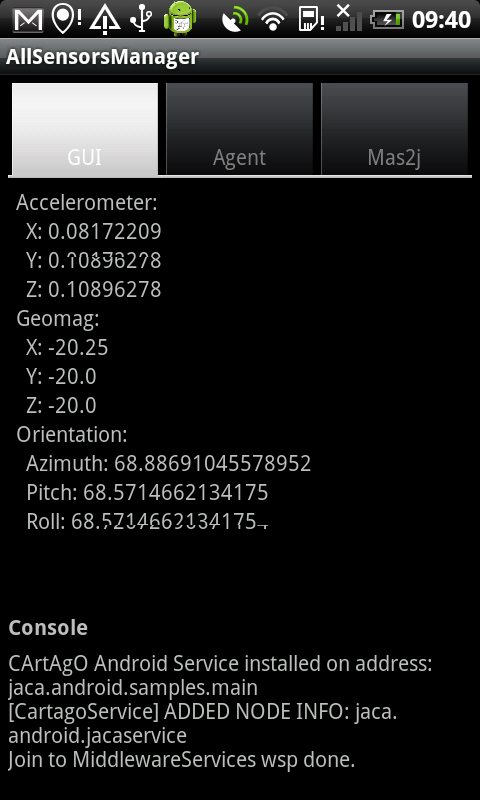
\includegraphics[width=8cm]{images/test_sensors_gui.png}
\end{center}
\caption{A screenshot of the described sample.}
\end{figure}

In \xt{test1agent} is reported the source code of the agent using the \mbox{\textsf{AllSensorManager}} artifact. 
%
Agent highlights: 

\begin{itemize}
%
\item The agent use the \code{init} plan for joining the \textsf{MiddlewareServices} workspace for having access to the \textsf{AllSensorManager} artifact.
%
\item Once joined the \textsf{MiddlewareServices} workspace the agents starts its job (plan \textsf{do\_job}) waiting for the \textsf{AllSensorManager} to be available (\code{focusWhenAvailable("all-sensors-manager")}).
%
\item Once focused the \textsf{AllSensorManager} artifact the behaviour of the agent is entirely managed by a set of reactive plans related to updates of the artifact's observable properties. As soon as a new sensors values are available the \textsf{AllSensorManager} retrieves this values and then updates its observable properties accordingly (through the \code{onSensorChanged} internal operation). The agent reacts to these observable properties changes updating the GUI with the new values (\code{updateAccSensorsInfo}, \code{updateGeomagSensorsInfo} and \code{updateOrientationSensorsInfo} operations provided by the artifact representing the application GUI).
%
\end{itemize}


%%%%%%%%%%%%%%%%%%%%%%%%%%%%%%%%%%%%%%%%%%%%%%%%%%%%%%%%%%%%%%%%%%%%%%%%%%%%%%%%%%%%%%%%%%%%%%%%%%%%%%%%%%%%%%%%%%%%%%%%%%%%%%%%%%%%%%%%%%%%%%%%%%%
\section{Example 02 - Working with the GPS}
%%%%%%%%%%%%%%%%%%%%%%%%%%%%%%%%%%%%%%%%%%%%%%%%%%%%%%%%%%%%%%%%%%%%%%%%%%%%%%%%%%%%%%%%%%%%%%%%%%%%%%%%%%%%%%%%%%%%%%%%%%%%%%%%%%%%%%%%%%%%%%%%%%%

In this example we will show how to work with the GPS in \textsf{JaCa-Android}. You can find the source code of this sample in the folder \code{/jaca/android/tests/gps} placed inside the main \code{tests} folder. 

The agent used in this sample joins the \textsf{MiddlewareServices} workspace for working with the \textsf{GPSManager} artifact, an artifact provided by the middleware that encapsulates the access to the device's GPS.  The \textsf{GPSManager} artifact is an artifact extending the \textsf{LocationManagerArtifact}, a \textsf{JaCa-Android} artifact that provides basic functionalities for managing the device's geographical location.
%
The artifact has a set of observable properties (\code{latitude}, \code{longitude}, \code{altitude}, \code{bearing}, etc.) that make directly accessible to agents the information coming from the GPS. 
%
These observable properties are dynamically updated by the artifact, by means of the usual linking mechanism between Android events -- GPS-related events in this case -- and artifact operations as described previously. 

\begin{table}[!ht]
\begin{tabular} {p{10cm}}
\begin{minipage}{10cm}
{\scriptsize \begin{verbatim}

public class GPSManager extends LocationManagerArtifact {

  protected void init(int minTime, int minDistance) {
    super.init(minTime, minDistance);
    linkOnLocationChangedEventToOp(LocationManager.GPS_PROVIDER, 
      "onLocationChange");
    Location location = getLocationManager()
                          .getLastKnownLocation(LocationManager.GPS_PROVIDER);
    if (location!=null) {
      defineObsProperty(LATITUDE, location.getLatitude());
      defineObsProperty(LONGITUDE, location.getLongitude());
      defineObsProperty(ALTITUDE, location.getAltitude());
      ...
    } else {
      defineObsProperty(LATITUDE, 0);
      defineObsProperty(LONGITUDE, 0);
      ...
    }
  }
		
  protected void dispose() {
    super.dispose();
    removeLocationUpdates(LocationManager.GPS_PROVIDER);
  }
	
  @INTERNAL_OPERATION void onLocationChange(Location arg0) {
    signal(ON_LOCATION_CHANGE, arg0.getProvider());
    getObsProperty(LATITUDE).updateValue(arg0.getLatitude());
    getObsProperty(LONGITUDE).updateValue(arg0.getLongitude());
    ...
  }
}
\end{verbatim}}
\end{minipage}
\end{tabular}
\caption{Source code snippet of the \textsf{GPSManager}.}
    \labeltab{GPSManager}
\end{table}


In \xt{GPSManager} is reported a source code snippet of the \textsf{GPSManager} artifact.\textsf{GPSManager} highlights:
\begin{itemize}
%
\item In the initialisation phase: \textit{(i)} the definition of the artifact observable properties (for the full list see the artifact's source code), \textit{(ii)} the linking between the gps-related events and the artifact operations responsible of the handling of such events.
%
\item The observable properties are updated as soon as new gps information are retrieved from the device's GPS. This is done inside the \code{onLocationChange} internal operation that, thanks to the link done in the \code{init}, is called each time new sensors values are available.
%
\item The generation of appropriate signals each time the artifact starts/ends receiving gps-related events. The start/end of the monitoring of such events is handled by the \code{startMonitoring}/\code{stopMonitoring} operations inherited from the \code{LocationManagerArtifact}.
\end{itemize}

\begin{table}[!ht]
\begin{tabular} {p{10cm}}
\begin{minipage}{10cm}
{\scriptsize \begin{verbatim}
!start.

+!start
  <-  !init;
      !do_job.

/*Initialisation plan for joining the MiddlewareServices workspace*/
+!init 
  <-  ...
	
/************************* Main agent plan ************************/		
+!do_job : wsp_id(jaca_services, WspID) & art_id(console,LocalConsoleID)
  <-  focusWhenAvailable("gps-manager")[wsp_id(WspID)];
      startMonitoring[wsp_id(WspID)];
      println("Ready.")[artifact_id(LocalConsoleID)].
		
+latitude(Latitude) : art_id(console,LocalConsoleID)
  <-  println("Latitude: ", Latitude)[artifact_id(LocalConsoleID)].
  
+longitude(Longitude) : art_id(console,LocalConsoleID)
  <-  println("Longitude: ", Longitude)[artifact_id(LocalConsoleID)].
	
+altitude(Altitude) : art_id(console,LocalConsoleID)
  <-  println("altitude: ", Altitude)[artifact_id(LocalConsoleID)].

...

\end{verbatim}}
\end{minipage}
\end{tabular}
\caption{Source code snippet of the \jason{} agent used in this test.}
    \labeltab{test2agent}
\end{table}

In \xt{test2agent} is reported the source code of the agent using the \textsf{GPSManager} artifact. Agent highlights:
\begin{itemize}
\item For first the agent joins the \textsf{MiddlewareServices} workspace using the usual \code{init} plan.
%
\item Then the agent focuses the \code{GPSManager}, contained in the \textsf{MiddlewareServices} workspace, and then invokes the \code{startMonitoring} operation on such artifact for starting receiving the information coming from the device's GPS.
%
\item Updates to the \code{GPSManager} observable properties are managed by a set of reactive plans in which the agent simply prints in the console the new information coming from the \textsf{GPSManager}.
\end{itemize}

\clearpage
\begin{figure}[!h]
\begin{center}
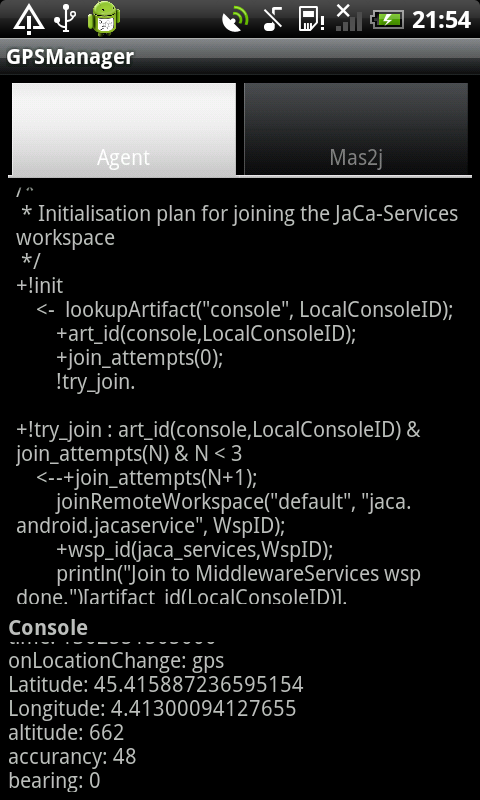
\includegraphics[width=8cm]{images/test_gps_gui.png}
\end{center}
\caption{A screenshot of the GPS sample in action.}
\end{figure}


%%%%%%%%%%%%%%%%%%%%%%%%%%%%%%%%%%%%%%%%%%%%%%%%%%%%%%%%%%%%%%%%%%%%%%%%%%%%%%%%%%%%%%%%%%%%%%%%%%%%%%%%%%%%%%%%%%%%%%%%%%%%%%%%%%%%%%%%%%%%%%%%%%%
\section{Example 03 - Reading the battery status}
%%%%%%%%%%%%%%%%%%%%%%%%%%%%%%%%%%%%%%%%%%%%%%%%%%%%%%%%%%%%%%%%%%%%%%%%%%%%%%%%%%%%%%%%%%%%%%%%%%%%%%%%%%%%%%%%%%%%%%%%%%%%%%%%%%%%%%%%%%%%%%%%%%%

In this example we will show how to retrieve information related to the device battery in \jacandroid{}. You can find the source code of this sample in the folder \code{/jaca/android/tests/battery} placed inside the main \code{tests} folder. The agent used in this sample joins the \textsf{MiddlewareServices} workspace for working with the \textsf{BatteryArtifact} artifact, an artifact provided by the middleware that allows to retrieve information about the device's battery. 


\begin{table}[!ht]
\begin{tabular} {p{10cm}}
\begin{minipage}{10cm}
{\scriptsize \begin{verbatim}
public class BatteryArtifact extends BroadcastReceiverArtifact {
	
  ...
	
  protected void init(boolean abortBroadcast) {
    super.init();
    defineObsProperty(HEALT, HEALT_GOOD);
    defineObsProperty(STATUS, "ok");
    defineObsProperty(LEVEL, 100);
    IntentFilter filter = new IntentFilter();
    filter.addAction(BATTERY_CHANGED);
    IntentFilter filter2 = new IntentFilter();
    filter.addAction(BATTERY_LOW);
    IntentFilter filter3 = new IntentFilter();
    filter3.addAction(BATTERY_OK);
    linkBroadcastReceiverToOp(filter, "batteryInfoReceived", abortBroadcast);
    linkBroadcastReceiverToOp(filter2, "batteryLowReceived", abortBroadcast);
    linkBroadcastReceiverToOp(filter3, "batteryOkReceived", abortBroadcast);
  }
	
  @INTERNAL_OPERATION public void batteryOkReceived(BroadcastReceiver broadcastReceiver, 
     Context context, Intent intent) {
    getObsProperty(STATUS).updateValue(STATUS_OK);
  }

  @INTERNAL_OPERATION public void batteryLowReceived(BroadcastReceiver broadcastReceiver, 
      Context context, Intent intent) {
    getObsProperty(STATUS).updateValue(STATUS_LOW);
  }
	
  @INTERNAL_OPERATION public void batteryInfoReceived(BroadcastReceiver broadcastReceiver, 
    Context context, Intent intent) {
    if (intent.getAction().equals(BATTERY_CHANGED)) {
      int level = intent.getIntExtra(BatteryManager.EXTRA_LEVEL, 100);
      getObsProperty(LEVEL).updateValue(level);
      int healt = intent.getIntExtra(BatteryManager.EXTRA_HEALTH, 
         BatteryManager.BATTERY_HEALTH_GOOD);
      String obsHealt = getObsProperty(HEALT).stringValue();

      if(healt!=BatteryManager.BATTERY_HEALTH_GOOD && obsHealt.equals(HEALT_GOOD))
        getObsProperty(HEALT).updateValue(HEALT_DEAD);
      else if(healt!=BatteryManager.BATTERY_HEALTH_DEAD && obsHealt.equals(HEALT_DEAD))
        getObsProperty(HEALT).updateValue(HEALT_GOOD);
    } 
  }
	
  protected void dispose(){
    super.dispose();
    unlinkBroadcastReceiverToOp(OP_BATTERY_INFO_RECEIVED);
    ...
  }
}
\end{verbatim}}
\end{minipage}
\end{tabular}
\caption{Source code snippet of the \textsf{BatteryArtifact}.}
    \labeltab{BatteryArtifact}
\end{table}

The \textsf{BatteryArtifact} is an artifact extending the \keyword{BroadcastReceiverArtifact}, a \textsf{JaCa-Android} artifact that provides basic functionalities for registering an artifact as the target of Android broadcasts, in this case broadcasts concerning battery information updates. Roughly speaking the \keyword{BroadcastReceiverArtifact} can be considered as the \jacandroid{} version of the classical Android \keyword{BroadcastReceiver}.


In \xt{BatteryArtifact} is reported a source code snippet of the \textsf{BatteryArtifact}.
%
\textsf{BatteryArtifact} highlights:
\begin{itemize}
%
\item In the artifact initialisation we create the observable properties related to the battery level, status and health (namely the \code{battery\_level}, the \code{battery\_status} and the \code{battery\_health}) and then we register the artifact to be notified by the broadcasts of interest for continuously retrieving updates related to the battery status.
%
\item In the artifact disposal we call the \code{unlinkBroadcastReceiverToOp} method (inherited by the \code{BroadcastReceiverArtifact}) for unregister the artifact, during its disposal, as one of the target to be notified by battery broadcasts.
\end{itemize}

\begin{table}[!ht]
\begin{tabular} {p{10cm}}
\begin{minipage}{10cm}
{\scriptsize \begin{verbatim}
!start.

+!start
  <-  !init;
      !do_job.

/*Initialisation plan for joining the MiddlewareServices workspace*/
+!init 
  <-  ...
		
/************************* Main agent plan ************************/		
+!do_job : wsp_id(jaca_services,WspID) & art_id(console,LocalConsoleID)
  <-  focusWhenAvailable("battery-artifact")[wsp_id(WspID)];
      println("Ready.")[artifact_id(LocalConsoleID)].

/********** Plans that handle reactions to battery events **********/
+battery_level(Value) : art_id(console,LocalConsoleID)
  <-  println("Battery level is ", Value)[artifact_id(LocalConsoleID)].

+battery_status(Value) : art_id(console,LocalConsoleID)
  <-  println("Battery status is ", Value)[artifact_id(LocalConsoleID)].

+battery_healt(Value) : art_id(console,LocalConsoleID)
  <-  println("Battery healt is ", Value)[artifact_id(LocalConsoleID)].
	
\end{verbatim}}
\end{minipage}
\end{tabular}
\caption{Source code snippet of the \jason{} agent used in this test.}
    \labeltab{test3agent}
\end{table}

In \xt{test3agent} is reported the source code of the agent using the \mbox{\textsf{BatteryArtifact}} artifact. Agent highlights:
\begin{itemize}
%
\item For first the agent joins the \textsf{MiddlewareServices} workspace using the usual \code{init} plan.
%
\item Then the agent focus the \code{BatteryArtifact}, contained in the \mbox{\textsf{MiddlewareServices}}, for receiving the information related to the battery.
%
\item As soon as new battery information are available the \code{BatteryArtifact} generates proper signals that are handled by the agent with a set of reactive plans that prints in the console the new battery information.
\end{itemize}

\clearpage
\begin{figure}[h!]
\begin{center}
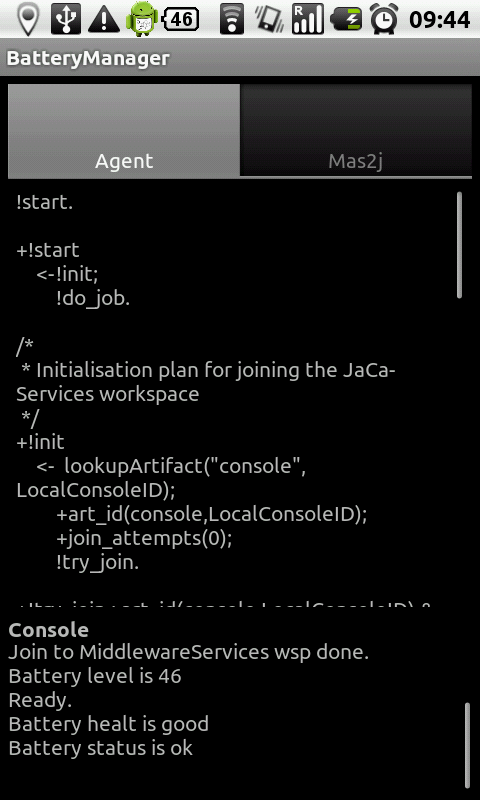
\includegraphics[width=8cm]{images/test_battery_gui.png}
\end{center}
\caption{A screenshot of the described sample.}
\end{figure}
\clearpage
%%%%%%%%%%%%%%%%%%%%%%%%%%%%%%%%%%%%%%%%%%%%%%%%%%%%%%%%%%%%%%%%%%%%%%%%%%%%%%%%%%%%%%%%%%%%%%%%%%%%%%%%%%%%%%%%%%%%%%%%%%%%%%%%%%%%%%%%%%%%%%%%%%%
\section{Example 04 - Working with the device connectivity}
%%%%%%%%%%%%%%%%%%%%%%%%%%%%%%%%%%%%%%%%%%%%%%%%%%%%%%%%%%%%%%%%%%%%%%%%%%%%%%%%%%%%%%%%%%%%%%%%%%%%%%%%%%%%%%%%%%%%%%%%%%%%%%%%%%%%%%%%%%%%%%%%%%%

In this example we will show how to manage the different kind of connectivity available on the device in \jacandroid{}. You can find the source code of this example in the folder \code{/jaca/android/tests/connectivity} placed inside the main \code{tests} folder. The agent used in this sample joins the \mbox{\textsf{MiddlewareServices}} workspace for working with the \mbox{\textsf{ConnectivityManager}} artifact, an artifact provided by the middleware that allows to manage the different kind of connectivity available on the device. Even if this artifact is meant to be able to manage all the different kind of connectivity available, currently, besides the management of the device airplane mode, only the WiFi is supported. This artifact, like the \textsf{BatteryArtifact}, extends the \textsf{BroadcastReceiverArtifact} for receiving the Android's broadcast (i.e. changes in the connectivity status in this case).



\begin{table}[!htp]
\begin{tabular} {p{10cm}}
\begin{minipage}{10cm}
{\scriptsize \begin{verbatim}

public class ConnectivityManager extends BroadcastReceiverArtifact {
	
  protected void init() {
    super.init();
    boolean isAirplaneEnabled = ...

    wifiManager = (WifiManager) getApplicationContext().getSystemService(Context.WIFI_SERVICE);
		
    if(isAirplaneEnabled)
      defineObsProperty(AIRPLANE_MODE_STATUS, ON_VALUE);
    else
      defineObsProperty(AIRPLANE_MODE_STATUS, OFF_VALUE);
		
    if(wifiManager.isWifiEnabled())
      defineObsProperty(WIFI_STATUS, ON_VALUE);
    else
      defineObsProperty(WIFI_STATUS, OFF_VALUE);
		
    IntentFilter filter = new IntentFilter();
    filter.addAction("android.intent.action.SERVICE_STATE");
    filter.addAction(WifiManager.WIFI_STATE_CHANGED_ACTION);
    linkBroadcastReceiverToOp(filter, "onReceive");
	}
	
	@INTERNAL_OPERATION void onReceive(BroadcastReceiver broadcastReceiver, 
	    Context context, Intent intent) {
    boolean isAirplaneEnabled = ...
    boolean obsIsAirplaneOn = getObsProperty(AIRPLANE_MODE_STATUS).equals(ON_VALUE);
    boolean obsIsWifiOn = getObsProperty(WIFI_STATUS).equals(ON_VALUE);
		
    if(obsIsAirplaneOn!=isAirplaneEnabled){
      if(isAirplaneEnabled)
        getObsProperty(AIRPLANE_MODE_STATUS).updateValue(ON_VALUE);
      else
        getObsProperty(AIRPLANE_MODE_STATUS).updateValue(OFF_VALUE);
    }
    if(obsIsWifiOn!=wifiManager.isWifiEnabled()){
      if(obsIsWifiOn)
        getObsProperty(WIFI_STATUS).updateValue(ON_VALUE);
      else
        getObsProperty(WIFI_STATUS).updateValue(OFF_VALUE);
    }
  }
	
  @OPERATION public void enableWiFi(){...}

  @OPERATION public void disableWiFi(){...}

  @OPERATION void enableAirplaneMode(){...}
	
  @OPERATION void disableAirplaneMode(){...}
  ...
}
\end{verbatim}}
\end{minipage}
\end{tabular}
\caption{Source code snippet of the \textsf{ConnectivityManager}.}
    \labeltab{ConnectivityManager}
\end{table}


In \xt{ConnectivityManager} is reported a source code snippet of the \textsf{ConnectivityManager} artifact.
%
\textsf{ConnectivityManager} highlights:

\begin{itemize}
%
\item In the artifact initialisation we create the observable properties related to the device's connectivity status and then we register the artifact to be notified by the broadcasts of interest for continuously retrieving updates related to such status.
%
\item Thanks to the usual linking mechanism between android events and artifacts' internal operations each time a new Android broadcast is sent the \code{onReceive} operation is invoked. Inside this operation the artifact's observable properties are updated with the last broadcasted information.
%
\item The artifact provides also a set of operations for: \textit{(i)} enabling/disabling the WiFi connectivity, and\textit{ (ii)} enabling/disabling the airplane-mode\footnote{This is the Android term used for indicating a device with at least cellular network turned off.} on the device.

\end{itemize}

In \xt{test4agent} is reported the source code of the agent used in this example.
%
Agent highlights:

\begin{itemize}
%
\item For first the agent joins the \textsf{MiddlewareServices} workspace using the usual \code{init} plan.
%
\item Then the agent focuses the \code{ConnectivityManager}, contained in the \textsf{MiddlewareServices}, for receiving the information related to the device connectivity status.
%
\item As soon as new information are available the \code{ConnectivityManager} generates proper signals that are handled by the agent with a set of reactive plans that print in the console the new connectivity information.
%
\item Inside the \code{do\_job} plan we test the different functionalities provided by the \code{ConnectivityManager} artifact enabling and then disabling the WiFi connection and the airplane mode.
\end{itemize}

\begin{figure}[!ht]
\begin{center}
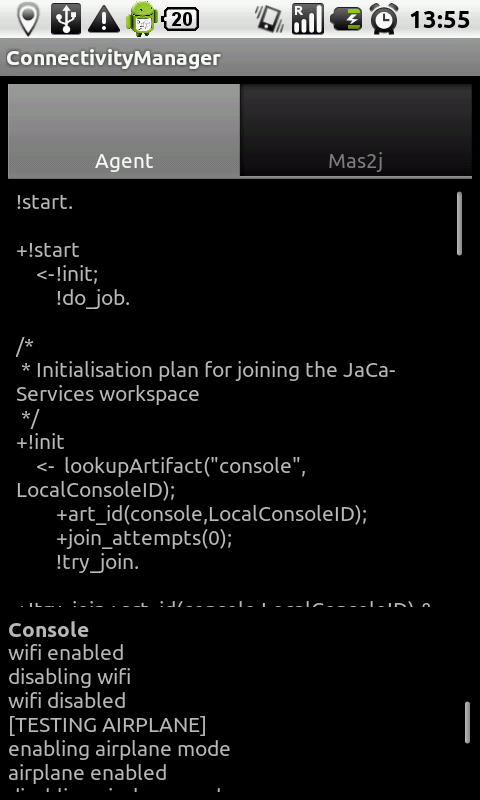
\includegraphics[width=6cm]{images/test_connectivity_gui.png}
\end{center}
\caption{A screenshot of the described sample.}
\end{figure}

\clearpage

\begin{table}[!h]
\begin{tabular} {p{10cm}}
\begin{minipage}{10cm}
{\scriptsize \begin{verbatim}

!start.

+!start
  <-  !init;
      !do_job.

/*Initialisation plan for joining the MiddlewareServices workspace*/
+!init 
  <-  ...
		
/******************** Main agent plan ********************/		
+!do_job : wsp_id(jaca_services, WspID) & art_id(console,LocalConsoleID)
  <-  focusWhenAvailable("connectivity-manager")[wsp_id(WspID)];
      println("[TESTING WIFI]")[artifact_id(LocalConsoleID)];
      !test_wifi;
      .wait(10000);
      println("[TESTING AIRPLANE]")[artifact_id(LocalConsoleID)];
      !test_airplane;
      .wait(10000);
      println("[DISABLE ALL]")[artifact_id(LocalConsoleID)];
      !disable_all.
		
+!test_wifi : true
  <-  ?art_id(console,LocalConsoleID);
      println("enabling wifi")[artifact_id(LocalConsoleID)];
      enableWiFi;
      println("wifi enabled")[artifact_id(LocalConsoleID)];
      .wait(15000);
      println("disabling wifi")[artifact_id(LocalConsoleID)];
      disableWiFi;
      println("wifi disabled")[artifact_id(LocalConsoleID)].
	   

+!test_airplane : true
  <-  ?art_id(console,LocalConsoleID);
      println("enabling airplane mode")[artifact_id(LocalConsoleID)];
      enableAirplaneMode;
      println("airplane enabled")[artifact_id(LocalConsoleID)];
      .wait(10000);
      println("disabling airplane mode")[artifact_id(LocalConsoleID)];
      disableAirplaneMode;
      println("airplane disabled")[artifact_id(LocalConsoleID)].

+!disable_all : true
  <-  ?art_id(console,LocalConsoleID);
      println("disabling all")[artifact_id(LocalConsoleID)];
      enableAirplaneSpecific("cell,bluetooth,wifi");
      println("all disabled")[artifact_id(LocalConsoleID)].
	
+airplane_mode_status(Value) : art_id(console,LocalConsoleID)
  <-  println("[STATUS AIRPLANE:]", Value)[artifact_id(LocalConsoleID)].
	
+wifi_status(Value) :art_id(console,LocalConsoleID)
  <-  println("[STATUS WIFI:]: ", Value)[artifact_id(LocalConsoleID)].
\end{verbatim}}
\end{minipage}
\end{tabular}
\caption{Source code snippet of the \jason{} agent used in this test.}
    \labeltab{test4agent}
\end{table}
\clearpage
%%%%%%%%%%%%%%%%%%%%%%%%%%%%%%%%%%%%%%%%%%%%%%%%%%%%%%%%%%%%%%%%%%%%%%%%%%%%%%%%%%%%%%%%%%%%%%%%%%%%%%%%%%%%%%%%%%%%%%%%%%%%%%%%%%%%%%%%%%%%%%%%%%%
\section{Example 05 - Working in remote \jacandroid{} workspaces}\labelsec{remotewsp-android}
%%%%%%%%%%%%%%%%%%%%%%%%%%%%%%%%%%%%%%%%%%%%%%%%%%%%%%%%%%%%%%%%%%%%%%%%%%%%%%%%%%%%%%%%%%%%%%%%%%%%%%%%%%%%%%%%%%%%%%%%%%%%%%%%%%%%%%%%%%%%%%%%%%%

In this example we will show how it is possible to realise a \jacandroid{} application that works also in a remote \jacandroid{} workspace (so a workspace related to another \jacandroid{} application). You can find the source code of this example in the folder \code{/jaca/android/tests/remotewsp/android} placed inside the main \code{tests} folder. 
%

Before launching this example is needed to install and run the \code{[JaCa-Android]RemoteWsp.apk} application contained in the \code{utils-projects/remote-android} folder on the root of the standard \jacandroid{} distribution. This apk contains a simple \jacandroid{} application (the application is composed by a \textsf{Calculator} artifact and a test agent that uses the artifact for performing basic computations) configured for being reachable by external \jacandroid{} applications. 


A \jacandroid{} application reachable from others ones can be realised in the following way. For first is necessary to configure the \textsf{JaCaService} in the Android manifest as reported below:

{\scriptsize \begin{verbatim}
  <service android:name="jaca.android.JaCaService" android:exported="true" >
    <intent-filter>
      <!-- 
          The action is the "Android address" that we want to expose as a remote wsp. 
          In the mas2j MUST be provided the same address when installing the 
          infrastructure: service(android,"remote.myaddress")
      -->
      <action android:name="remote.myaddress" />
      <category android:name="android.intent.category.DEFAULT" />
    </intent-filter>
  </service>
\end{verbatim}}

\noindent Then in the \code{mas2j} configuration file we need to create an environment of type \code{CartagoEnvironment} as reported below:
%
%
{\scriptsize \begin{verbatim}
MAS remote_wsp {
	
	infrastructure: Centralised

    environment: 
      c4jason.CartagoEnvironment("infrastructure", service(android,"remote.myaddress"))

    agents: agent agentArchClass c4jason.CAgentArch;

    aslSourcePath: "test/remote";
}
\end{verbatim}}
%
\noindent In this way, when we launch this application we also install a \cartago{} node (of type \code{infrastructure}) that, thanks to the \code{service(android,"remote.myaddress")} parameter, makes the application reachable by external \jacandroid{} ones at the address \code{remote.myaddress}. The \cartago{} infrastructure will use the configuration just described for allowing other applications to communicate with the remote one using the infrastructure protocol specified (so in this case means using the \cartago{} infrastructure protocol that relies on Android IPC). For further details please refer to the \cartago{} website\footnote{\url{http://cartago.sourceforge.net/?page_id=139}}.
%
Please note that the address specified in the \textsf{mas2j} \textbf{must} be the same as the one specified in the \code{JaCaService} inside the Android manifest file.


Our test application is composed by a simple agent that join the default workspace of the \code{[JaCa-Android]RemoteWsp.apk} application and then starts to use the \textsf{Calculator} artifact contained in it printing the obtained result in the local console and in the remote one. For making our test application able to reach the remote workspaces its \textsf{mas2j} file must be configured as reported below:

{\scriptsize \begin{verbatim}

MAS test {
	
	infrastructure: Centralised

   environment: c4jason.CartagoEnvironment("standalone", protocol(android))

    agents:  
   		agent agentArchClass c4jason.CAgentArch;

    aslSourcePath: "jaca/android/tests/remotewsp/android";
}
\end{verbatim}}


\noindent The configuration for the \code{CartagoEnvironment} specifies that this application will not be reachable from the outside (\code{standalone} parameter) but that it will be able to join remote workspaces through the Android infrastructure protocol (\code{protocol(android)} parameter).


In \xt{remote-agent1} is reported the source code of the agent used in this test.
%
Agent highlights:

\begin{itemize}
%
\item The test provides some facilitations that allow the user to insert the address (\code{remote.myaddress} in our case) to join from a GUI (thanks to the \code{AddressActivity}) and to memorise the address provided (thanks to the \code{Config} artifact). For sake of simplicity we are not reporting here details about the implementation of these facilitations.
%
\item Once the address has been setted the agent try to join the remote workspace thanks to the \code{joinRemoteWorkspace} action (\code{joinRemoteWorkspace("default", Address, RemoteWspId)}). In case of error during the connection a proper \jason{} recovery plan is instantiated (\code{-!join\_remote\_wsp}) and the \code{AddressActivity} is displayed again for letting the user insert a new address for the remote join.
%
\item Once the \code{joinRemoteWorkspace} succeeds the \code{work\_in\_remote\_wsp} plan is instantiated. Within this plan the agent works with the remote \code{Calculator} artifact and prints the result of its computation in both the local and the remote console.
%
\end{itemize}

\begin{figure}[!hb]
\begin{center}
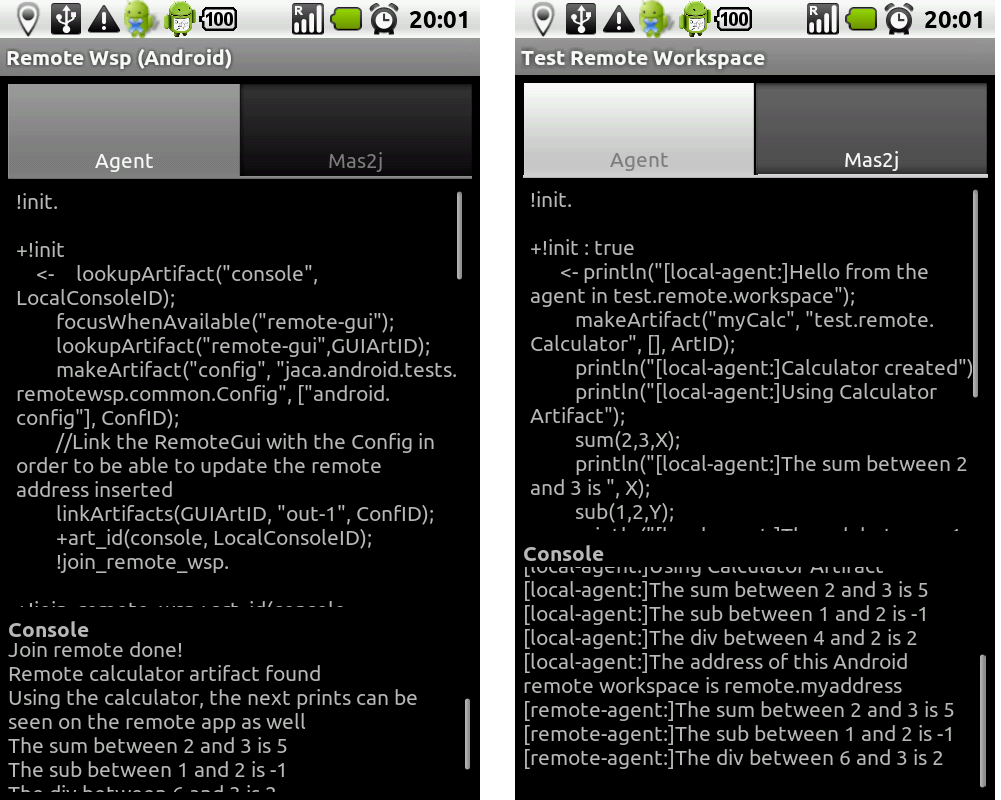
\includegraphics[width=.9\linewidth]{images/test_remote1_gui.png}
\end{center}
\caption{A screenshot of the described sample with in evidence the prints produced in both the local and remote application.}
\labelfig{remote1}
\end{figure}
\clearpage

\begin{table}[!ht]
\begin{tabular} {p{10cm}}
\begin{minipage}{10cm}
{\scriptsize \begin{verbatim}
!init.

+!init 
  <-  lookupArtifact("console",LocalConsoleID);
      focusWhenAvailable("remote-gui");
      lookupArtifact("remote-gui",GUIArtID);
      makeArtifact("config", "jaca.android.tests.remotewsp.common.Config", 
        ["android.config"], ConfID);
      linkArtifacts(GUIArtID, "out-1", ConfID);
      +art_id(console, LocalConsoleID);
      !join_remote_wsp.
	
+!join_remote_wsp : art_id(console, LocalConsoleID)
  <-  getAddress(Address);
    //Address not setted yet, we start the activity for obtaining the address
    if (Address == "") {
      startExplicitActivityForResult("jaca.android.tests.remotewsp.common.AddressActivity", 0);
    //Address setted, we try to join the remote wsp
    } else {
      joinRemoteWorkspace("default", Address, RemoteWspId); 
      +remote_wsp(RemoteWspId);
      println("Join remote done!")[artifact_id(LocalConsoleID)];
      !work_in_remote_wsp;
    }.

//Failure in joining the remote wsp: we ask again for the address
-!join_remote_wsp : true
  <-  startExplicitActivityForResult("jaca.android.tests.remotewsp.common.AddressActivity", 0).

/*Signal received by the RemoteGUI: the user has inserted the remote address,
 we can re-instantiate the join_remote_wsp plan */
+address_setted  :  true
  <-  !join_remote_wsp.
	
+!work_in_remote_wsp : art_id(console, LocalConsoleID)
	<-  lookupArtifact("myCalc", CalcId)[wsp_id(RemoteWspId)];
      lookupArtifact("console", RemoteConsoleID)[wsp_id(RemoteWspId)];
      println("Remote calculator artifact found")[artifact_id(LocalConsoleID)];
      println("Using the calculator, the next prints can 
         be seen on the remote app as well")[artifact_id(LocalConsoleID)];
      sum(2,3,X);
      println("[remote-agent:]The sum between 2 and 3 is ", X)[artifact_id(RemoteConsoleID)];
      println("The sum between 2 and 3 is ", X)[artifact_id(LocalConsoleID)];
      sub(1,2,Y);
      println("[remote-agent:]The sub between 1 and 2 is ", Y)[artifact_id(RemoteConsoleID)];
      println("The sub between 1 and 2 is ", Y)[artifact_id(LocalConsoleID)];
      division(6,3,Z);
      println("[remote-agent:]The div between 6 and 3 is ", Z)[artifact_id(RemoteConsoleID)];
      println("The div between 6 and 3 is ", Z)[artifact_id(LocalConsoleID)].
\end{verbatim}}
\end{minipage}
\end{tabular}
\caption{Source code snippet of the \jason{} agent used in this test.}
    \labeltab{remote-agent1}
\end{table}

%%%%%%%%%%%%%%%%%%%%%%%%%%%%%%%%%%%%%%%%%%%%%%%%%%%%%%%%%%%%%%%%%%%%%%%%%%%%%%%%%%%%%%%%%%%%%%%%%%%%%%%%%%%%%%%%%%%%%%%%%%%%%%%%%%%%%%%%%%%%%%%%%%%
\section{Example 06 - Working with standard \jaca{} remote workspace}
%%%%%%%%%%%%%%%%%%%%%%%%%%%%%%%%%%%%%%%%%%%%%%%%%%%%%%%%%%%%%%%%%%%%%%%%%%%%%%%%%%%%%%%%%%%%%%%%%%%%%%%%%%%%%%%%%%%%%%%%%%%%%%%%%%%%%%%%%%%%%%%%%%%
In this example we will show how it is possible to realise a \jacandroid{} application that works also in a remote \jaca{} workspace (so a workspace related to another \jaca{} application). You can find the source code of this example in the folder \code{/jaca/android/tests/remotewsp/lipermi} placed inside the main \code{tests} folder.


Before running this test you need to launch the \jaca{} application contained inside the \code{utils-projects/[JaCa]RemoteWsp} folder. 
%
Once inside that folder you will find the \code{\textsf{mas2j}} for launching the application inside the \code{src/test/remote} folder.
%
The \code{[JaCa]RemoteWsp} application is a \jaca{} version of exactly the same application used in the previous test (so an application composed by a \code{Calculator} artifact and a simple agent using it).

Note that \jacandroid{} applications can communicate with remote \jaca{} ones thanks to a \cartago{} infrastructure protocol that is \code{lipermi}-based. \code{lipermi}\footnote{\url{http://lipermi.sourceforge.net/}} is a library for managing remote method invocation in Java on top the TCP/IP protocol. Therefore for being able to run this sample you must run the \code{[JaCa]RemoteWsp} application from an IP node reachable from the Android device.

A \jaca{} application reachable from others ones using the \code{lipermi} infrastructure protocol can be realised simply configuring the \textsf{mas2j} file as follow (for further details see the \cartago{} website\footnote{\url{http://cartago.sourceforge.net/?page_id=139}}) :

\begin{table}[!h]
\begin{tabular} {p{10cm}}
\begin{minipage}{10cm}
{\scriptsize \begin{verbatim}
MAS remote_wsp{
	
	infrastructure: Centralised

    environment: c4jason.CartagoEnvironment("infrastructure", service(lipermi))

    agents: agent agentArchClass c4jason.CAgentArch;
    
    classpath : "../../../lib/*.jar";
}
\end{verbatim}}
\end{minipage}
\end{tabular}
\caption{\textsf{mas2j} configuration for a \jaca{} application reachable from remote ones through the \code{lipermi} infrastructure protocol.}
    \labeltab{remote-app21}
\end{table}



This \textsf{mas2j} configuration differ from the previous one just for the \code{service} parameter. In this case the infrastructure protocol that we use for joining and working with the remote workspace is the \code{lipermi} protocol. In the previous case we used the Android protocol but here we can not use it as our infrastructure protocol since the remote application in this case is not Android-based. Moreover we are not specifying an explicit address for the application, indeed in this case the remote address will be defined by the IP address of the machine where we will run the remote application followed by the default port for the \cartago{} \code{lipermi} infrastructure protocol (20101).
%

In this test, like the previous one, we use a simple agent that join the default workspace of the \code{[JaCa]RemoteWsp} application and then start to use the \textsf{Calculator} artifact contained in it printing the obtained results in the local console and in the remote one. 

\noindent For making our test application able to reach the remote workspaces its \textsf{mas2j} file must be configured as follow:


\begin{table}[!h]
\begin{tabular} {p{10cm}}
\begin{minipage}{10cm}
{\scriptsize \begin{verbatim}
MAS test {
	
	infrastructure: Centralised

    environment: c4jason.CartagoEnvironment("standalone", protocol(lipermi)) 

    agents:  
   		agent agentArchClass c4jason.CAgentArch;

    aslSourcePath: "jaca/android/tests/remotewsp/lipermi";
}
\end{verbatim}}
\end{minipage}
\end{tabular}
\caption{\textsf{mas2j} configuration for a \jacandroid{} application able to reach remote \jaca{} ones -- even \jacandroid{} ones -- through the \code{lipermi} infrastructure protocol.}
    \labeltab{remote-join2}
\end{table}



The configuration for the \code{CartagoEnvironment} specify that this application will not be reachable from the outside (\code{standalone} parameter) but that it will be able to join remote workspace through the lipermi infrastructure protocol (\code{protocol(lipermi)} parameter).


%
\noindent Agent Highlights:

\begin{itemize}
%
\item The source code of the agent is exactly the same as the one used in the previous test (and for this reason we are not reporting it here). Is the underlying \cartago{} infrastructure that manages the interaction with the remote application accordingly with the protocol specified in the \textsf{mas2j} configuration.
%
\item Our \jacandroid{} application differ from the one used in the previous test only in the configuration of the \textsf{mas2j} file. Indeed the only thing we need to change is the protocol to use for joining the remote workspace.
%
\item It is quite simple to realise \jacandroid{} application that can interact with other \jaca{} ones distributed in other network nodes. The same procedure can be used for joining remote applications running inside LANs or remote internet nodes.
%
\end{itemize}
 

\begin{figure}[h!]
\begin{center}
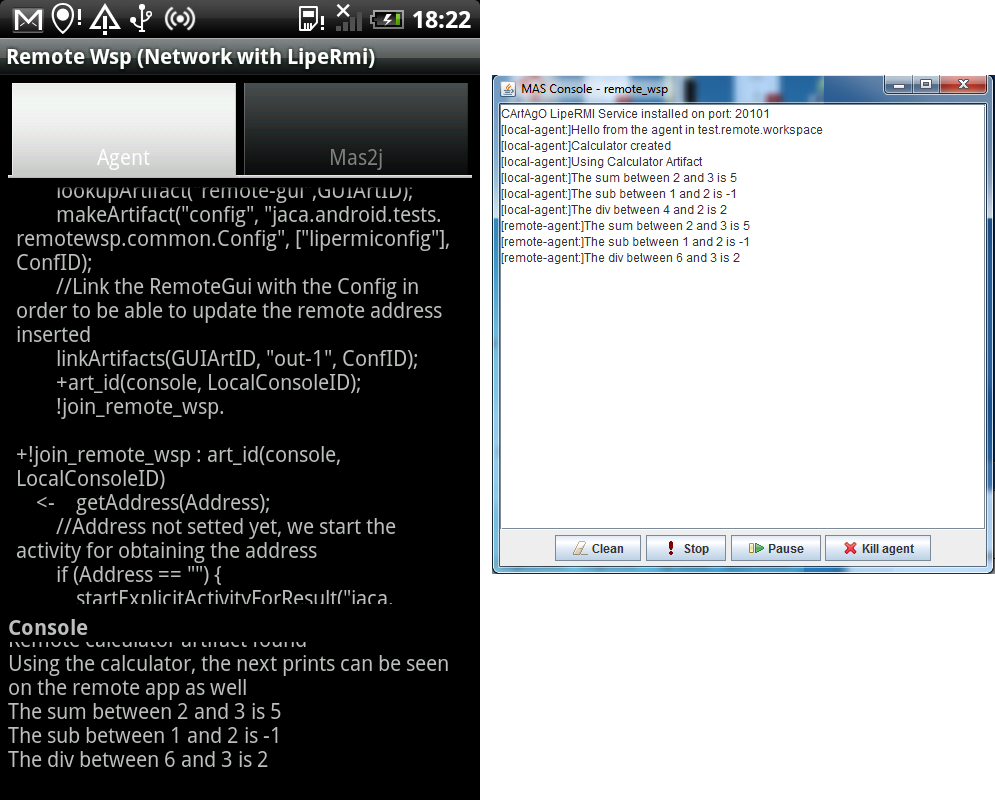
\includegraphics[width=.9\linewidth]{images/test_remote2_gui.png}
\end{center}
\caption{A screenshot of the described sample with in evidence the prints produced in both the local and remote application.}
\labelfig{remote2}
\end{figure}



\chapter{Examples}
\tbc{}
\section{Context-aware SMS notifier}
\tbc{}
\section{JaCa-Locale}
\tbc{}
\chapter{Performance tests}
\tbc{}
\section{Reactivity test}
\tbc{}
\section{Memory occupation test}
\tbc{}
\section{Heavy computation test}

\bibliography{bib}
\bibliographystyle{abbrv}

\end{document}
	